% ================================================================== PART III
\part{The virtual experiment}

\chapter{Test flows, synthetic PIV and error metrics}
To measure the error of a reconstruction we need flows whose pressure is known exactly. The project uses two exact Navier--Stokes solutions (plus a convected variant) and a CFD simulation, then degrades their velocity like a real PIV system.

\begin{figure}[H]\centering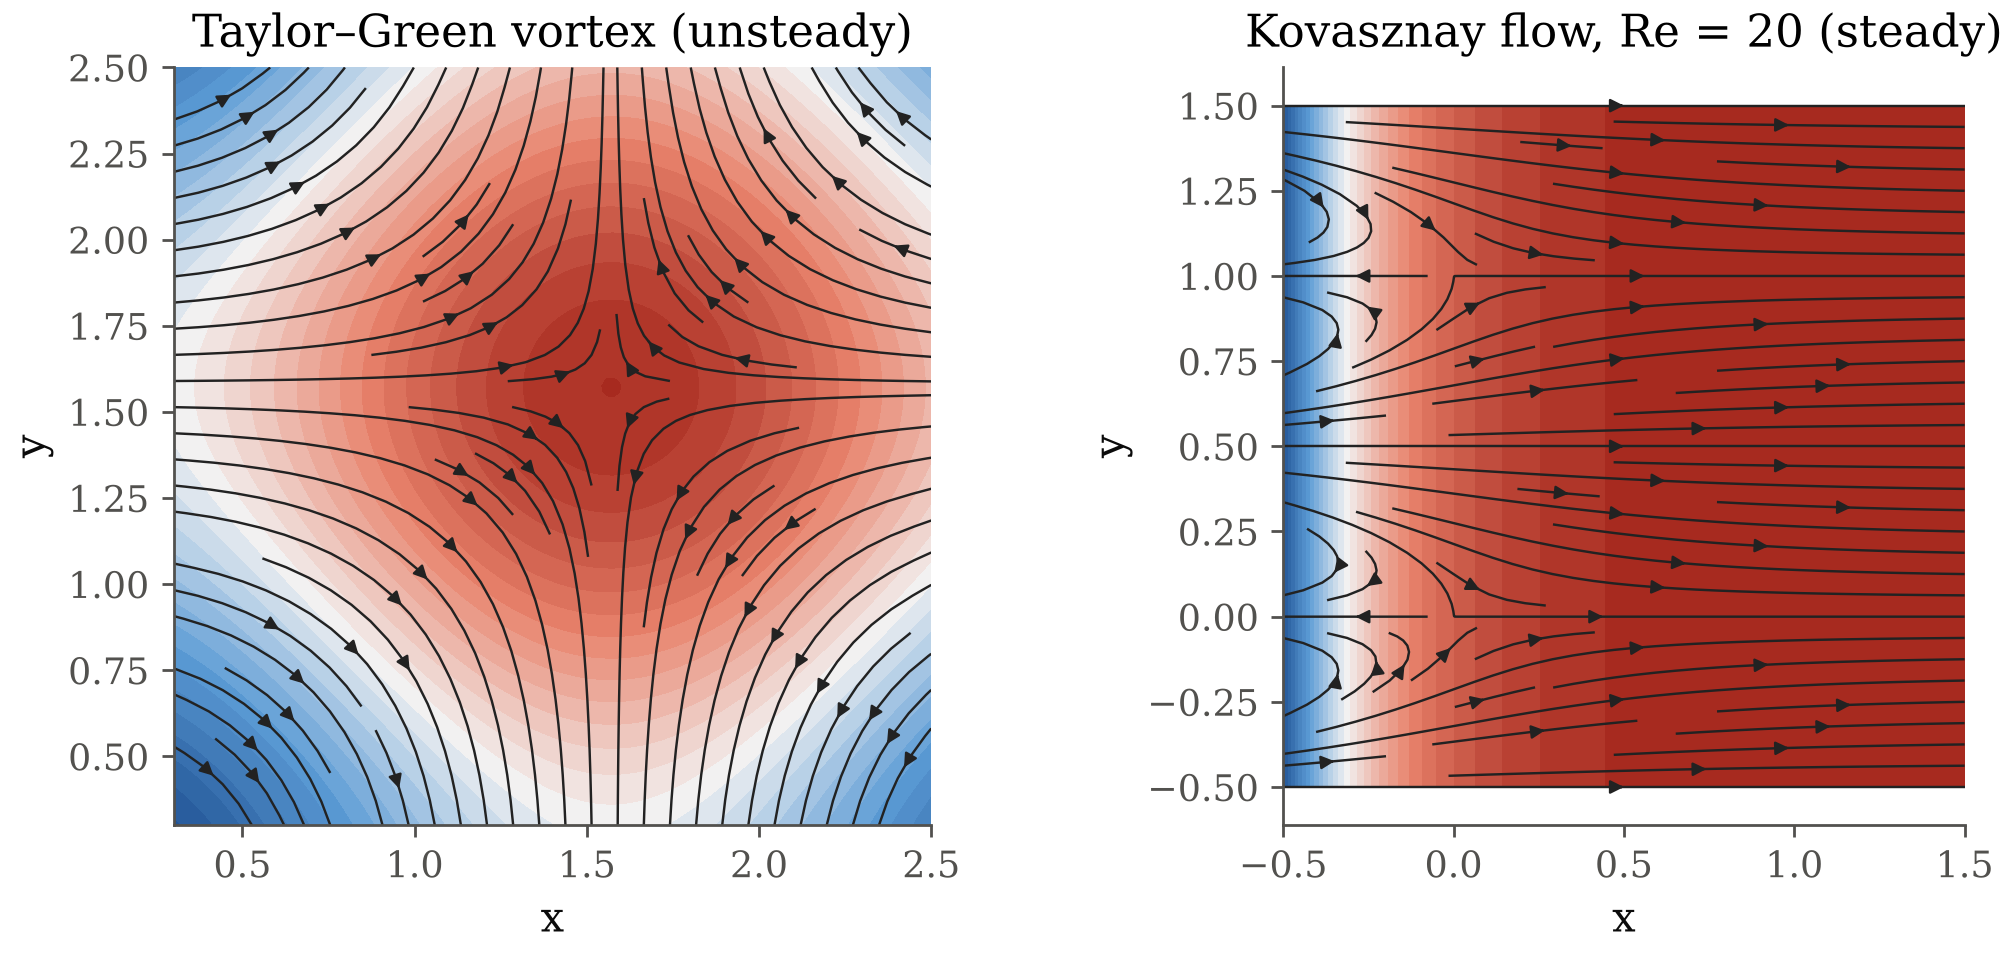
\includegraphics[width=0.85\linewidth]{img/f_testcases.png}
\caption{The two exact test flows: pressure (colour) and streamlines. Left: Taylor--Green on the window $[0.3,2.5]^2$. Right: Kovasznay flow at Re = 20 on $[-0.5,1.5]^2$.}\end{figure}

\section{Taylor--Green vortex}
\begin{equation}
u=\cos x\sin y\,F(t),\quad v=-\sin x\cos y\,F(t),\quad p=-\tfrac{\rho}{4}(\cos2x+\cos2y)F(t)^2,\quad F=e^{-2\nu t}.
\end{equation}
\textbf{Why it is exact.} Each velocity component is an eigenfunction of the Laplacian, $\nabla^2u=-2u$, so $\partial\uu/\partial t=-2\nu\uu=\nu\nabla^2\uu$: the unsteady and viscous terms cancel exactly. The convective term is then a pure gradient, balanced by $-\nabla p/\rho$:
\[
(\uu\cdot\nabla)\uu=\tfrac12\big(\sin2x,\;\sin2y\big)F^2=-\nabla p/\rho .
\]
So $\G=\nabla p$ comes entirely from convection: a good test of the convective term.

\textbf{Settings.} $\nu=0.01$, snapshots at $t=1\pm\Delta t$ with $\Delta t=0.05$.
\begin{itemize}
\item \textbf{Main window} $[0.3,2.5]^2$: deliberately non-periodic, so the Neumann boundary treatment is actually tested (on a full period the boundary terms would cancel).
\item \textbf{Core window} $[\pi-1.1,\pi+1.1]^2$: the main window contains no vortex core (its centre is a saddle, a pressure maximum), so vortex-core metrics use this second window centred on the core at $(\pi,\pi)$.
\end{itemize}

\textbf{Convected Taylor--Green.} Navier--Stokes is Galilean invariant: if $(\uu,p)$ is a solution, so is $\uu'(\mathbf x,t)=\mathbf c+\uu(\mathbf x-\mathbf ct,t)$, $p'=p(\mathbf x-\mathbf ct,t)$. With amplitude $A=0.4$ and $\mathbf c=(1,0)$ the vortex pattern is swept through the window, so $\partial\uu/\partial t=O(1)$ as in a real wake. This is the case where the Eulerian/Lagrangian comparison is meaningful (vortex speed $w=0.4$ < convection speed $c=1$).

\section{Kovasznay flow}
Kovasznay (1948) found an exact steady solution resembling the flow behind a grid:
\begin{equation}
u=1-e^{\lambda x}\cos2\pi y,\quad v=\frac{\lambda}{2\pi}e^{\lambda x}\sin2\pi y,\quad p=\frac{\rho}{2}\left(1-e^{2\lambda x}\right),\quad \lambda=\frac{Re}{2}-\sqrt{\frac{Re^2}{4}+4\pi^2}.
\end{equation}
\begin{itemize}
\item Continuity: $u_x=-\lambda e^{\lambda x}\cos2\pi y$ and $v_y=\lambda e^{\lambda x}\cos2\pi y$ cancel. \checkmark
\item Substituting into the steady equations gives $\lambda^2-Re\,\lambda-4\pi^2=0$; the negative root gives a wake that decays downstream: $\lambda\approx-1.81$ at Re = 20 and $-0.96$ at Re = 40.
\item The flow is steady, so $D\uu/Dt=(\uu\cdot\nabla)\uu$, and $\mu=\rho/Re$ is large: the viscous term matters. Kovasznay therefore tests the viscous term, which Taylor--Green does not.
\item Its pressure depends on $x$ only, with a steep gradient near the inflow edge $x=-0.5$.
\end{itemize}

\section{The synthetic PIV model}
\code{piv/degrade.py} turns an exact field into PIV-like data in three steps, applied in this order:
\begin{enumerate}
\item \textbf{Interrogation-window averaging.} The truth is sampled 4$\times$ finer than the PIV grid (with a margin), and a box filter of width $W$ is applied to $u$ and $v$ of every snapshot. For even widths the plain moving average would be off-centre by half a cell; the code averages the two half-shifted windows, which gives a centred trapezoidal box of width exactly $W$.
\item \textbf{Subsampling} to the PIV spacing $h$ (every 4th fine node), then cropping the margin, so the PIV nodes are exactly \code{linspace(x0, x1, n)}.
\item \textbf{Noise.} Independent Gaussian noise $N(0,(\sigma U)^2)$ on $u$ and $v$ at every node and snapshot, with a fixed seed.
\end{enumerate}
The \emph{reference pressure is never filtered}: it is only subsampled, so the measured error includes the bias that window averaging causes.

\textbf{Baseline.} $64\times64$ vectors, $W=h$, $\sigma=1\,\%$ of $U$, $\Delta t=0.05$. Each study varies one parameter around this baseline.

\begin{pitfall}[Fixed noise level across window sizes]
In real PIV a larger window contains more particles, so its random error is \emph{smaller}. The model keeps $\sigma$ fixed (as the project specification asked), so here $W$ only adds bias. Making $\sigma$ decrease with $W$ would reproduce the real resolution--noise trade-off; this is listed as future work.
\end{pitfall}

\section{Denoising}
Two optional filters act on $u$ and $v$ before differentiation:
\begin{itemize}
\item \textbf{Gaussian filter} (standard deviation 1 grid point): transfer function $e^{-(k s h)^2/2}$. It smooths everything, including real curvature.
\item \textbf{2-D Savitzky--Golay} ($5\times5$ window, quadratic): at each node, a least-squares fit of a polynomial in $x,y$, evaluated at the node (via the pseudo-inverse of the Vandermonde matrix). It reproduces quadratics exactly, also at the edges where the window is shifted inwards, so it biases smooth peaks less than the Gaussian.
\end{itemize}

\section{Error metrics}
Pressure is known only up to a constant, so both fields are demeaned first ($p'=p-\bar p$):
\begin{equation}
\eps_{L2}=\frac{\|p'-p'_{ref}\|_2}{\|p'_{ref}\|_2},\qquad
\eps_{max}=\frac{\max|p'-p'_{ref}|}{\tfrac12\rho U^2}.
\end{equation}
Also reported: the error map $|p'-p'_{ref}|$; a line profile through the vortex core; and the \textbf{core ratio}, reconstructed core pressure (minimum within $3h$ of the true core) divided by the true one. A ratio below 1 means the suction is under-predicted.

\section{Experiment design}
\begin{itemize}
\item \textbf{One factor at a time} around the baseline, so each effect is attributed cleanly (a local sensitivity study).
\item \textbf{Ten noise seeds} per point; results are mean $\pm$ standard deviation. The standard error of the mean falls as $1/\sqrt N$.
\item \textbf{Common random numbers:} the same seeds are reused across parameter values, so differences between parameter values are less noisy than the scatter itself.
\item Runs are deterministic: re-running reproduces every number.
\end{itemize}

% ------------------------------------------------------------------
\chapter{The code}

\section{Architecture}
\begin{figure}[H]
\centering
\begin{tikzpicture}[node distance=4mm and 6mm, every node/.style={font=\small\sffamily},
  mod/.style={draw=accent,fill=boxbg,rounded corners=2pt,align=left,text width=40mm,minimum height=9mm,inner sep=4pt},
  ar/.style={-{Stealth[length=2mm]},thick,color=accent!80!black}]
\node[mod] (fields) {\textbf{fields/}\\ FlowField, analytic, CFD loader};
\node[mod,right=of fields] (piv) {\textbf{piv/}\\ degrade, denoise};
\node[mod,right=of piv] (core) {\textbf{core/}\\ derivatives, $D\uu/Dt$, Poisson, direct, omni, iterative, \code{reconstruct()}};
\node[mod,below=of core] (an) {\textbf{analysis/}\\ metrics, norms, plots, summary};
\node[mod,left=of an] (st) {\textbf{studies/}\\ one script per sweep $\to$ CSV};
\node[mod,left=of st] (cfd) {\textbf{cfd/}\\ case generator, run scripts, export, grid independence};
\draw[ar] (fields)--(piv); \draw[ar] (piv)--(core); \draw[ar] (core)--(an); \draw[ar] (st)--(core); \draw[ar] (cfd)--(fields);
\end{tikzpicture}
\caption{Package structure. Every data source returns a \code{FlowField}; every algorithm consumes one.}
\end{figure}

\begin{itemize}
\item \textbf{\code{FlowField}} (\code{fields/field.py}) is the common interface: $x,y,t$ and arrays $u,v$ of shape $[n_t,n_y,n_x]$, plus $\rho$, $\mu$, the reference pressure and $U_{ref}$. It checks that the grids are uniform, because every stencil assumes constant spacing.
\item \textbf{\code{reconstruct()}} (\code{core/pipeline.py}) is the single entry point: it computes $\G$, then calls the chosen method, and returns the pressure plus diagnostics (compatibility residual, timings, solver history).
\item \textbf{\code{studies/}} contains one script per parameter sweep; each writes a CSV row per reconstruction and saves its figures.
\item \textbf{\code{analysis/summary.py}} writes \code{results/SUMMARY.md} from the CSVs, so no number in the report is typed by hand.
\end{itemize}

\section{Pseudo-code}
\begin{lstlisting}
for case in [TaylorGreen, ConvectedTG, Kovasznay20, Kovasznay40, CFD]:
    truth = exact_or_cfd(case)                 # u, v, p on a 4x finer grid
    for param in sweep(h | sigma | dt | BC | method | W | filter):
        for seed in range(10):
            F  = degrade(truth, W, h, sigma, seed)  # box filter, subsample, noise
            F  = denoise(F)                     # optional
            a  = DuDt(F, eulerian | lagrangian)
            G  = -rho*a + mu*lap(u)
            p  = poisson(G) | direct(G) | omni(G)
            eps  = L2(p' - p'_ref) / L2(p'_ref)   # p' = p - mean(p)
        save mean, std of eps -> CSV -> figures -> SUMMARY.md
\end{lstlisting}

\section{Inside the Poisson solve}
\begin{lstlisting}
f = div(G)                                  # or -rho(u_x^2 + 2 u_y v_x + v_y^2)
b = f + ghost-point terms +/-2G/h on the edges (both at corners)
R = trapz(f) - contour(n.G)                 # compatibility residual, reported
if Dirichlet edges:   rows -> p_k = value
elif pin == "node":   row k -> p_k = 0
else:                 solve [[A, 1], [1^T, 0]] [p, lam] = [b, 0]   # zero mean
p = spsolve(...)   or   Jacobi / GS / SOR / CG on the same system
\end{lstlisting}

\section{Tests: how we know the code is right}
87 unit tests (\code{python -m pytest -q}, about 15\,s) check every component against an exact answer:
\begin{itemize}
\item \textbf{Derivatives:} second-order slopes in the max norm, including boundary nodes; exact on quadratics and cubics.
\item \textbf{Poisson:} the manufactured solution $p=\sin x\cos y$ converges at order 2 for pin-mean, pin-node, direct and CG; the null space, $w^TA=0$, symmetry of $WA$, and the discrete compatibility identity.
\item \textbf{Taylor--Green and Kovasznay:} $\G=+\nabla p$ to second order; full reconstruction second order for all three methods; without $\mu\nabla^2\uu$ Kovasznay does not converge.
\item \textbf{Methods:} all exact for linear $p$; agree on clean data; noisy data show path dependence and omni/Poisson beat a single path.
\item \textbf{PIV model and I/O:} box filter centred and normalised; noise seeding; Savitzky--Golay preserves quadratics; OpenFOAM export parsers; Strouhal number from a synthetic force file; Richardson extrapolation recovers order 2.
\item \textbf{Convergence add-on:} norms (the lecture example), Jacobi = pseudo-time, classic-Jacobi stall, SOR divergence, all iterative solvers match \code{spsolve}, slope $\approx1$ for \code{order=1} and $\approx2$ for \code{order=2}.
\end{itemize}

\begin{viva}
\begin{enumerate}[leftmargin=*]
\item \emph{Why generate the truth finer than the PIV grid?} A PIV vector is an average over the window, so the underlying field must be resolved below $h$.
\item \emph{Why fixed seeds?} Reproducibility, and common random numbers make differences between parameter values less noisy.
\item \emph{How do you test second order?} Halve $h$ repeatedly and fit the slope of $\log\eps$ against $\log h$; the tests accept 1.8--2.3 because coarse grids are pre-asymptotic.
\item \emph{Why a common \code{FlowField}?} Degradation, integration and metrics need not know whether data are analytic, CFD or turbulence-database data.
\end{enumerate}
\end{viva}
